\documentclass[a4paper]{ctexart}
\usepackage{syntonly}
%令LaTeX编译后不生成PDF文档,只排查错误,编译速度会快不少
\usepackage{amsmath,amssymb,amsfonts,bm,varwidth,enumitem,cases,graphicx,float,subfigure,siunitx}
%graphicx支持插图
%array对表格列格式的扩展
%booktabs排版三线表
%amsmath,amssymb,amsfonts排版数学公式三件套
%mathtools数学公式扩展宏包,提供了公式编号定制和更多的符号、矩阵等
%cases提供numcases环境,在公式的每行case后面增加编号
%varwidth保持盒子的自然宽度
\usepackage[most]{tcolorbox}
%tcolorbox以TikZ为基础提供排版样式丰富的彩色盒子的功能,并加载大部分的库
\usepackage[mathstyleoff]{breqn}
%breqn自动对长的显示公式折行,且会随行宽而自动调整折行的位置,并启用安全模式
\usepackage[left=19.1mm,right=19.1mm,top=1in,bottom=1in]{geometry}
%geometry修改页边距参数
\ctexset{section/name={第,节}}
%修改章节编号的样式
\usepackage[pdftitle=平面几何讲义,colorlinks=true,linkcolor=black,bookmarksnumbered=false,pdfsubject=平面几何,pdfstartview=FitH]{hyperref}
%colorlinks=true为链接文字带颜色
%bookmarksnumbered=true书签带章节编号
%pdfauthor作者
%pdfsubject主题
%pdfstartview=FitH设置PDF页面以适合宽度的方式显示
\allowdisplaybreaks[4]%允许多行公式分页
\graphicspath{{figures/}}
\title{\bf{平面几何、解析几何讲义}}
\author{张杰骜\\2250368776@qq.com}
\date{\today}

\begin{document}
\maketitle%生成标题页
\begin{center}%---------------------------------------------------------
    
\includegraphics[scale=0.2]{0}
\end{center}%---------------------------------------------------------
\newpage
\tableofcontents%生成目录
\newpage
\raggedbottom%令页面在垂直方向向顶部对齐

%\section{圆的初步}
\subsection{四点共圆的判定}
四点共圆的条件:四点A,B,C,D共圆的充要条件为:$\angle{ABC}=\angle{ADC}\neq0$(同侧)
或$\angle{ABC}+\angle{ADC}=180^{\circ}$(异侧).

此外,相交弦定理逆定理,切割线定理逆定理,托勒密定理逆定理等许多关于圆的相关定理的逆定理
也都可作为四点共圆的判据,需要根据题目条件灵活使用(不过使用做多的还是利用角度进行判断)。

四点共圆在平几题中出现频率非常高,在问题中一般有两种形式:一是作为证题的目的;通常需要根据
题设条件推出判定四点共圆的条件(前述的几种),也可以用两组四点共圆来证明题设要求的四点共圆;
二是作为解题的工具,可以用于证明角相等、线垂直等。
\begin{figure}[H]
    \centering  
    \subfigure{
    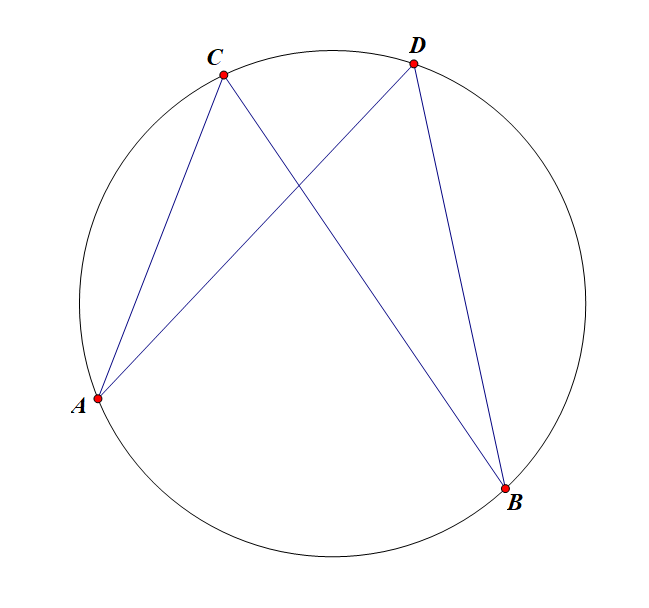
\includegraphics[scale=0.4]{4}}
    \subfigure{
    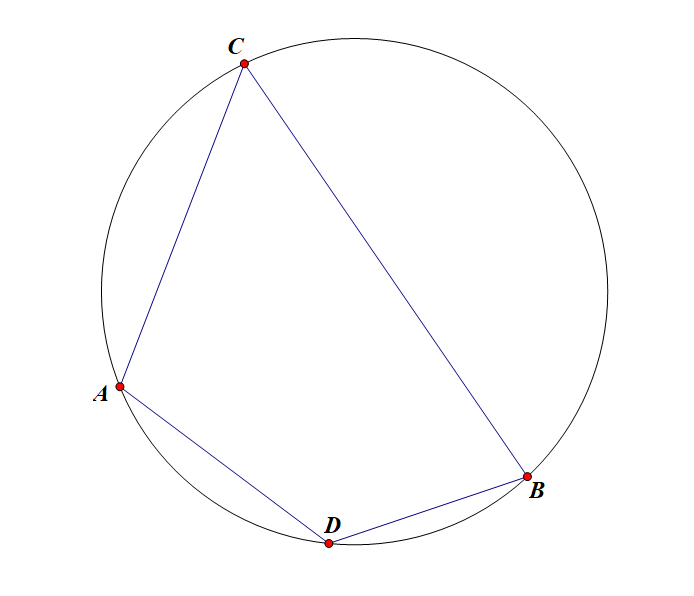
\includegraphics[scale=0.4]{5}}
\end{figure}
\subsection{与圆相关的定理}
(1)托勒密定理:在凸四边形ABCD中,$AB\cdot CD+AD\cdot BC\geq AC\cdot BD$,
当且仅当四边形ABCD是圆内接四边形时,等号成立。
\begin{center}
    \includegraphics*[scale=0.5]{1.png}
\end{center}

三弦定理:设PA,PB,PC是圆内一公共端点的三条弦,则
$$PA\sin{\angle{BPC}}+PC\sin{\angle{APB}}=PB\sin{\angle{APC}}$$

三弦定理逆定理:设PA,PB,PC是一公共端点的三条线段,若
$$PA\sin{\angle{BPC}}+PC\sin{\angle{APB}}=PB\sin{\angle{APC}}$$
则P,A,B,C四点共圆。
\begin{center}
    \includegraphics*[scale=0.3]{2.png}
\end{center}

(2)西姆松定理
过三角形外接圆上异于三角形顶点的任意一点作三边的垂线,则三垂足点共线(此线称为西姆松线)。
\begin{center}
    \includegraphics*[scale=0.5]{3.png}
\end{center}

(3)帕斯卡定理
圆内接六边形ABCDEF三组对边(延长线)的交点P、Q、R三点共线。
\begin{figure}[H]
    \centering  
    \subfigure{
    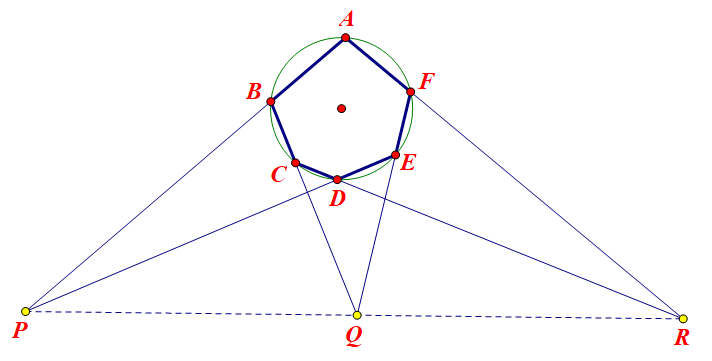
\includegraphics[scale=0.5]{6}}
    \subfigure{
    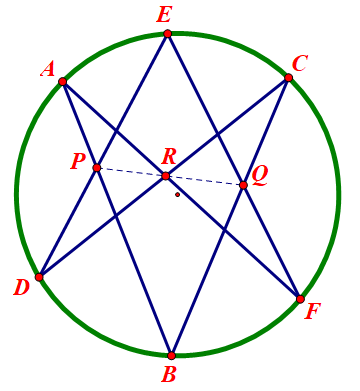
\includegraphics[scale=0.5]{7}}
\end{figure}
\newpage
\subsection{例题}
1.$\quad$ AB是圆O的直径.C与D是互异的圆O上的两点,且在AB的一侧.过C、D作圆的切线交于点E.线段AD与BC交于点F,直线EF交AB于M.求证:E,C,M,D四点共圆.
\begin{center}
    \includegraphics*[scale=0.4]{20}
\end{center}

~\\
~\\
~\\
~\\
~\\
~\\

2.A、B、C三点共线,O点在直线外。$O_1,O_2,O_3$分别
为$\bigtriangleup OAB,\bigtriangleup OBC,\bigtriangleup OCA$的外心.求证: 
$O,O_1,O_2,O_3$四点共圆.
\begin{center}
    \includegraphics*[scale=0.4]{21}
\end{center}
\newpage

3.$\bigtriangleup ABC$中,$AB=AC$,点E,F分别在AB,AC上,$AE<AF$,BF,CE交于点P.求证:$PF<PE$.
\begin{center}
    \includegraphics*[scale=0.4]{22}
\end{center}

~\\

4.圆O过$\bigtriangleup ABC$顶点A、C,且与AB、BC交于K、N(K、N不同).$\bigtriangleup ABC$外接圆和$\bigtriangleup BKN$外接圆交于B、M两点。求证:
$\angle{BMO}=90^{\circ}$.
\begin{center}
    \includegraphics*[scale=0.4]{23}
\end{center}


5.在平行四边形ABCD中,过点C作AB,AD的垂线CM,CN,垂足分别为M,N,MN,BD的延长线交于点P.求证:PC$\bot $AC.
\begin{center}
    \includegraphics*[scale=0.4]{24}
\end{center}


%\newpage
\section{三角形的五心}
\subsection{五心的定义与性质}
三角形的重心、垂心、内心、外心、旁心称为三角形的五心。


1.重心:三角形的三条中线交于一点,该点叫做三角形的重心;重心将每条中线都分成定比2:1。

$\bigtriangleup{ABC}$中线长度公式:
$$AD^2=\frac{1}{2}\sqrt{2AC^2+2AB^2-BC^2}$$,AD为中线。


2.外心:三角形外接圆的圆心,叫做三角形的外心。



3.垂心:三角形的三条高交于一点,该点叫做三角形的垂心。
\begin{center}
    \includegraphics*[scale=0.75]{8}
\end{center}

垂心的性质:

(1)三角形的三个顶点、三个垂足、垂心这7点可以得到6个四点圆,
三组相似三角形,且$AH\cdot HD=BH\cdot HE=CH\cdot HF$。

(2)H、A、B、C四点中任一点是其余三点为顶点的三角形的垂心,称为一垂心组。

(3)$\angle{BHC}=180^{\circ}-\angle{A}=\angle{B}+\angle{C}$

(4)O是外心,H是垂心,则$\angle{BAO}=\angle{HAC},\angle{ABO}=\angle{HBC}$

(5)H关于三边的对称点在$\bigtriangleup{ABC}$的外接圆上,关于
三边中点的对称点在$\bigtriangleup{ABC}$的外接圆上。

(6)三角形外心O、重心G、垂心H三点共线,且OG:GH=1:2(欧拉线)。

(7)三角形任一顶点到垂心的距离等于外心到对边距离的2倍。

(8)设$\bigtriangleup{ABC}$的垂心为H,外接圆半径为R,
则
$$
\frac{HA}{|\cos{A}|}=\frac{HB}{|\cos{B}|}=\frac{HC}{|\cos{C}|}=2R
$$

(9)三角形的垂心是其垂足三角形的内心。

九点圆:$\bigtriangleup{ABC}$三条高的垂足$D,E,F$,
三边中点$A_1,B_1,C_1$,以及顶点与
垂心H联线段的中点$A_2,B_2,C_2$九点共圆。
\begin{center}
    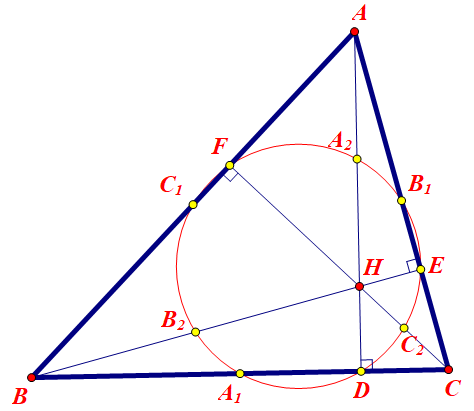
\includegraphics[scale=0.5]{9.png}
\end{center}

证明:
\begin{figure}[H]
    \centering  
    \subfigure{
        \begin{minipage}[t]{0.25\linewidth}
            \centering
            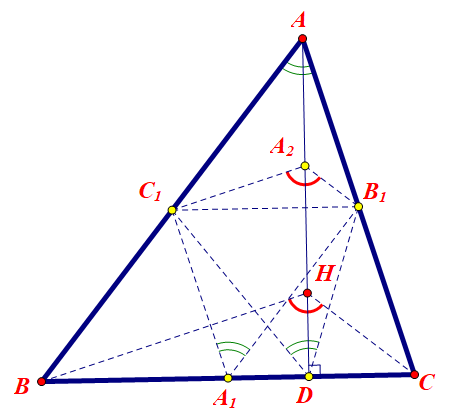
\includegraphics[scale=0.35]{10}
        \end{minipage}}
    \subfigure{
        \begin{minipage}[t]{0.25\linewidth}
            \centering
            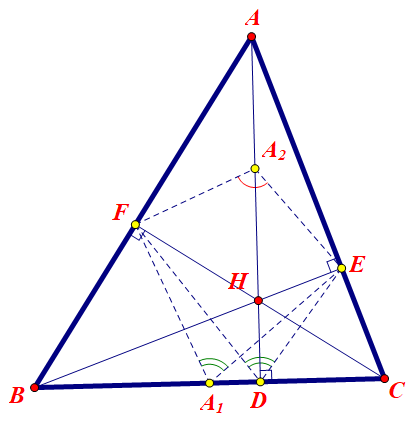
\includegraphics[scale=0.35]{11}
        \end{minipage}}
    \subfigure{
        \begin{minipage}[t]{0.25\linewidth}
            \centering
            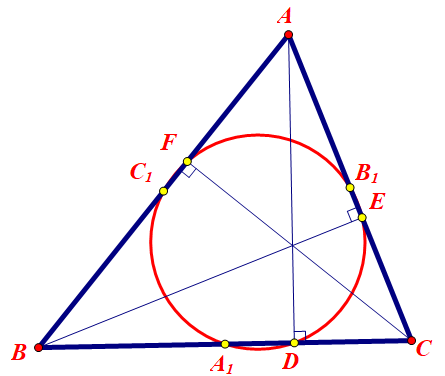
\includegraphics[scale=0.35]{12}
        \end{minipage}}
\end{figure}

位似性质:
\begin{center}
    \includegraphics*[scale=0.75]{13}
\end{center}
\newpage
4.内心:三角形内切圆的圆心,叫做三角形的内心(三角平分线的交点)。

性质:

(1)张角公式:$\angle{BIC}=90^{\circ}+\frac{1}{2}\angle{A}$


(2)设I为$\bigtriangleup ABC$的内心,$AI,BI,CI$分别交外接圆于$D,E,F$,则I为$\bigtriangleup{DEF}$的垂心。
\begin{center}
    \includegraphics*[scale=0.5]{15}
\end{center}

(3)设I为$\bigtriangleup ABC$的内心,$BC=a,AC=b,AB=c$,
$\angle{A}$的平分线交BC于K,交$\bigtriangleup ABC$的外接圆于点D,则
\[
    \frac{AI}{KI}=\frac{DI}{DK}=\frac{AD}{DI}=\frac{b+c}{a}
\]
\begin{center}
    \includegraphics*[scale=0.6]{16}
\end{center}

5.旁心:三角形的旁切圆的圆心,叫做三角形的旁心(三角形一内角平分线和另两顶点处的外角平分线的交点)

(1)鸡爪定理:设$I,I_1$分别是$\bigtriangleup{ABC}$的内心、旁心,延长AI交外接圆于S点,则
$$SI=SB=SC=SI_1$$
\begin{center}
    \includegraphics*[scale=0.5]{17}
\end{center}

(2)三角形的三个旁心与内心构成一垂心组。
\begin{figure}[H]
        \centering  
        \subfigure{
                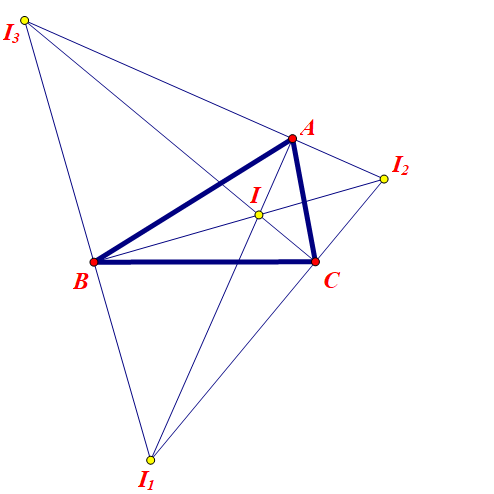
\includegraphics[scale=0.5]{18}}
        \subfigure{
                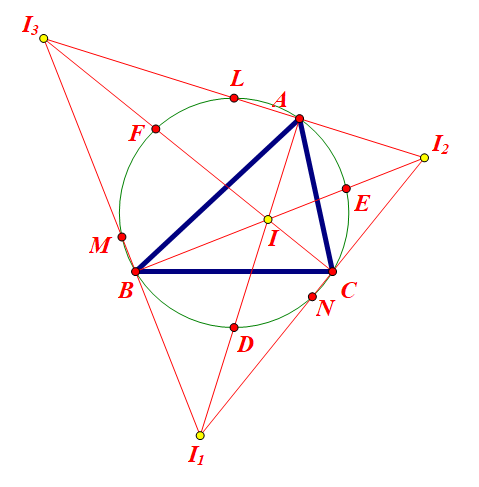
\includegraphics[scale=0.5]{19}}
\end{figure}

\subsection{例题}
1.设H为锐角三角形$\bigtriangleup ABC$的垂心,D为边BC的中点,过点H的直线分别交边AB、AC于点F、E,使得AE=AF,射线DH与$\bigtriangleup ABC$的外接圆交于P.求证:
P、A、E、F四点共圆.

\begin{center}
    \includegraphics*[scale=0.3]{25}
\end{center}

2.设点O是锐角三角形$\bigtriangleup ABC$的外心.分别以$\bigtriangleup ABC$三边的中点为圆心作过点O的圆,这三个圆两两的异于O的交点分别
为K、L、M.证明:点O是$\bigtriangleup KLM$的内心.
\begin{center}
    \includegraphics*[scale=0.3]{26}
\end{center}
\newpage
3.在$\bigtriangleup ABC$中,AB=AC,一个圆内切于$\bigtriangleup ABC$的外接圆$\odot O$于M,并与AB、AC分别相切于P、Q两点.I为线段PQ中点.求证:
I是$\bigtriangleup ABC$的内心.
\begin{center}
    \includegraphics*[scale=0.3]{27}
\end{center}

4.$AD$是直角三角形$ABC$斜边上的高,($AB<AC$),$I_1,I_2$分别是$\bigtriangleup ABD,\bigtriangleup ACD$的内心,$\bigtriangleup AI_1I_2$的外接圆$\odot O$分别交$AB,AC$
于$E,F$,直线$EF,BC$交于点$M$.证明:$I_1,I_2$分别是$\bigtriangleup ODM$的内心与旁心.
\begin{center}
    \includegraphics*[scale=0.4]{28}
\end{center}

5.$\bigtriangleup ABC$的内切圆$I$切$BC,AC$于$D,E$,$K,L$为$AB,AC$中点,证明:$BI,KL,DE$三线共点
\begin{center}
    \includegraphics*[scale=0.4]{29}
\end{center}
\newpage

6.在锐角三角形$ABC$中,$AB<AC$,$O$为外心,$H$为垂心。设直线$AO$与$BC$交于点$D$,点$E$在边BC上且满足$HE // AD$.证明:
$BE=CD$.
\begin{center}
    \includegraphics*[scale=0.4]{30}
\end{center}

7.例题3的推广:

(1)一般情形:设$\odot O'$与$\bigtriangleup ABC$外接圆切于点$D$,与$AB,AC$切于$E,F$点,$I$为线段$EF$中点.证明:$I$为
$\bigtriangleup ABC$的内心.
\begin{center}
    \includegraphics*[scale=0.4]{31}
\end{center}

(2)旁心情形:设$\odot O'$与$\bigtriangleup ABC$外接圆切于点$D$,与$AB,AC$的延长线切于$E,F$点,$I'$为线段$EF$中点.证明:$I'$为
$\bigtriangleup ABC$的$BC$边外的旁心.
\begin{center}
    \includegraphics*[scale=0.4]{32}
\end{center}

8.设$\bigtriangleup ABC$的垂心、外心分别为点$H,O$,BC的中垂线交$\bigtriangleup AOH$的外接圆于$A_1$,
($A_1\neq O$).类似定义点$B_1,C_1$。求证:$AA_1,BB_1,CC_1$三线共点.
\newpage
\section{圆中的比例线段、根轴}
\subsection{圆幂}
1.相交弦定理:圆内的两条相交弦被交点分成的两条线段的积相等。

2.切割线定理:从圆外一点引圆的切线和割线,切线长是这点到割线与圆交点的两条线段长
的比例中项

3.割线定理:从圆外一点引圆的两条割线,这一点到每条割线与圆的交点的两条线段长的积
相等

上述三个定理统称为圆幂定理:过一定点作两条直线与圆相交,则定点到每条直线与圆的交点的两条线段的
积相等,即它们的积为定值。
\begin{center}
    \includegraphics*[scale=0.4]{33}
\end{center}

4.点到圆的幂:点到圆心的距离为$d$,圆的半径为$r$,称$d^2-r^2$为定点到圆的幂。

当定点在圆内时,$d^2-r^2<0$

当定点在圆上时,$d^2-r^2=0$

当定点在圆外时,$d^2-r^2>0$

\subsection{根轴}
1.根轴:到两圆等幂的点的轨迹是与此二圆圆心连心线垂直的一条直线,这条直线称为两圆的根轴。

2.如果两圆相交,其根轴为两圆公共弦所在的直线。

3.如果两圆相切,其根轴就是过两圆切点的公切线。

4.三个圆,其两两的根轴或交于一点(根心),或互相平行。当三个圆两两相交时,三条公共弦所在的直线交于一点,
这一性质可以用于判断三线共点。
\begin{center}
    \includegraphics*[scale=0.3]{34}
\end{center}

\subsection{例题}
1.ABCD是圆$O$的内接四边形,延长$AB,DC$交于点$E$,
$EP,FQ$分别切圆$O$于$P,Q$.证明:$EP^2+FQ^2=EF^2$.

\begin{center}
    \includegraphics*[scale=0.3]{35}
\end{center}

2.自圆外一点P向圆O作切线PA、PB,A、B为切点,AB与PO
相交于C,弦EF过点C.证明:$\angle{APE}=\angle{BPF}$
\begin{center}
    \includegraphics*[scale=0.4]{36}
\end{center}

3.自圆外一点P向圆O引割线交圆于R、S两点,又作切线PA、PB,
A、B为切点,AB与PR相交于Q.证明:$\frac{1}{PR}+\frac{1}{PS}=\frac{2}{PQ}$
\begin{center}
    \includegraphics*[scale=0.35]{37}
\end{center}
\newpage
4.圆内接四边形ABCD的对角线交于点K,点M和N分别是
对角线AC和BD的中点,$\bigtriangleup ADM,\bigtriangleup BCM$的外接圆交于
点M、L,证明:K、L、M、N四点共圆.

~\\
~\\
~\\
~\\
~\\
~\\
~\\
~\\
~\\
~\\
~\\
~\\

5.$\bigtriangleup ABC$的内切圆与AB切于点C'
,设$\bigtriangleup ACC'$的内切圆分别与AB、AC切于点
$C_1,B_1$,$\bigtriangleup BCC'$的内切圆分别与AB、BC切于点$C_2,A_2$.
证明:$B_1C_1,A_2C_2,CC'$三线共点.
~\\
~\\
~\\
~\\
~\\
~\\
~\\
~\\
~\\
~\\
~\\

6.$\bigtriangleup ABC$中,E、F分别为AB、AC中点,CM、BN为高,
EF交MN于P,O、H分别为三角形的外心与垂心.证明:$AP\bot OH$.
\newpage

7.(欧拉定理)O、I分别为$\bigtriangleup ABC$的外心、内心,R、r分别为$\odot O,\odot I$的半径.
证明:$OI^2=R^2-2Rr$.
\begin{center}
    \includegraphics*[scale=0.5]{38}
\end{center}

8.已知D是$\bigtriangleup ABC$外接圆上任一点,作DE、DF与内切圆I都相切,交外接圆于E、F.
求证:EF也与内切圆I相切.
\begin{center}
    \includegraphics*[scale=0.5]{39}
\end{center}

9.$A_1A_2$是两个相离的圆$\odot O_1,\odot O_2$的外公切线,设$A_1A_2$的中点为$K$,过$K$作
$\odot O_1 ,\odot O_2$的切线$KB_1,KB_2$,$B_1,B_2$为切点.
直线$A_1B_1,A_2B_2$交于点$L$,直线$O_1O_2,KL$交于点$P$.
证明:$B_1,B_2,P,L$四点共圆.
\begin{center}
    \includegraphics*[scale=0.5]{40}
\end{center}
\newpage
\section{简单实战训练}
1.在$\bigtriangleup ABC$中,M是边AC的中点,D、E是$\bigtriangleup ABC$的外接圆在点A处的切线上的两点,
满足$MD//AB$,且A是线段DE的中点,过A、B、E三点的圆与边AC相交于另一点P,过
A、D、P三点的圆与DM延长线相交于点Q.证明:$\angle{BCQ}=\angle{BAC}$.
\begin{center}
    \includegraphics*[scale=0.35]{41}
\end{center}

2.如图所示,I是$\bigtriangleup ABC$的内心,点P、Q分别为I在边AB、AC上的投影,
直线PQ与$\bigtriangleup ABC$的外接圆相交于X、Y(P在X、Q之间)。已知
B、I、P、X四点共圆,证明:C、I、Q、Y四点共圆.
\begin{center}
    \includegraphics*[scale=0.35]{42}
\end{center}

3.如图,在$\bigtriangleup ABC$,$AB>AC$,$\bigtriangleup ABC$内两点X,Y均在$\angle{BAC}$的
平分线上,且满足$\angle{ABX}=\angle{ACY}$,设BX的延长线与线段CY交于点P,
$\bigtriangleup BPY$的外接圆与$\bigtriangleup CPY$的外接圆交于P与另一点
Q.证明:A、P、Q三点共线.
\begin{center}
    \includegraphics*[scale=0.35]{43}
\end{center}

4.如图所示,在锐角$\bigtriangleup ABC$中,$AB>AC$,M是$\bigtriangleup ABC$的外
接圆的劣弧$\hat{BC}$的中点,K是$\bigtriangleup BAC$的外角平分线与BC延长线的交点,在过点A且
垂直于BC的直线上取一点D(异于A),使得DM=AM.设$\bigtriangleup ADK$的外接圆与$\bigtriangleup ABC$外接圆相
交于点A及另一点T.证明:AT平分线段BC.
\begin{center}
    \includegraphics*[scale=0.35]{44}
\end{center}

5.如图,在等腰$\bigtriangleup ABC$中,$AB=BC$,I为内心,M为BI的中点,
P为边AC上一点,满足$AP=3PC$,PI延长线一点H满足$MH\perp PH$,Q为
$\bigtriangleup ABC$的外接圆上劣弧AB的中点.证明:$BH\perp QH$.
\begin{center}
    \includegraphics*[scale=0.30]{45}
\end{center}

6.如图,$\bigtriangleup ABC$为锐角三角形,AB<AC,M为BC边
的中点,点D和E分别为$\bigtriangleup ABC$的外接圆$\hat{BAC}$和$\hat{BC}$的中点,F为$\bigtriangleup ABC$的内
切圆在AB边上的切点,G为AE与BC的交点,N在线段EF上,满足$NB\perp AB$.
证明:若$BN=EM$,则$DF\perp FG$.
\begin{center}
    \includegraphics*[scale=1.0]{46}
\end{center}
\newpage
\section{平面几何中的常见方法——代数法、三角法}

\subsection{代数法常用定理与结论}

比例线段、切线长公式(内心,旁心)、角平分线定理、梅涅劳斯定理、塞瓦定理、托勒密定理、
圆幂定理、调和性质等等。(还有一些几何结构中表现出的与线段长、线段比例相关的性质)

\subsection{代数法例题}
1.已知O、I分别为$\bigtriangleup ABC$的外心和内心,$BC=a,CA=b,AB=c$.问当且仅当$a,b,c$满足什么条件时,有$OI\perp BI$.
\begin{flushleft}
    \includegraphics*[scale=0.5]{51}
\end{flushleft}
~\\
~\\
~\\


2.AD是$\bigtriangleup ABC\angle BAC$的外角平分线,并交$\bigtriangleup ABC$的外界圆
于D,以CD为直径的圆分别交BC,AC于P,Q.证明:线段PQ把$\bigtriangleup ABC$的周长二等分.
\begin{flushleft}
    \includegraphics*[scale=0.5]{47}
\end{flushleft}
~\\
~\\
\newpage

3.$\bigtriangleup ABC$中,BE、CF为AC、AB边上的高,$FP\perp BC$于P,$FQ\perp AC$于Q,
$EM\perp BC$于M,$EN\perp AB$于N,且$FP+FQ=CF,\quad EM+EN=BE$.证明:$\bigtriangleup ABC$
为正三角形.
\begin{flushleft}
    \includegraphics*[scale=0.5]{48}
\end{flushleft}
~\\
~\\



4.设AB是$\odot O$的直径,过点A、B的切线分别为$l_a,l_b$,C是
圆周上任意一点,BC交$l_a$于K,$\angle CAK$的平分线交CK于H.设M是弧CAB的中点,
HM与$\odot O$交于点S,过点M的切线与$l_b$交于点T.证明:S、T、K三点共线.
\begin{flushleft}
    \includegraphics*[scale=0.5]{49}
\end{flushleft}
~\\
~\\
~\\

\subsection{三角法}
1.常用方法与公式:正弦定理、余弦定理、积化和差、和差化积、三倍角公式、三弦定理、张角定理等.

2.三角形中的恒等式:
\begin{equation*}
    \cos^2 A+\cos^2 B+\cos^2 C=1-2\cos A \cos B \cos C 
\end{equation*}

\begin{equation*}
    \tan A+\tan B+\tan C=\tan A \tan B \tan C
\end{equation*}

\begin{equation*}
    \tan{\frac{A}{2}} \tan{\frac{B}{2}}+\tan{\frac{B}{2}} \tan{\frac{C}{2}}+\tan{\frac{A}{2}} \tan{\frac{C}{2}}=1
\end{equation*}

3.设$r,R$分别为$\bigtriangleup ABC$的内切圆、外接圆半径,则有
\begin{equation*}
    \frac{r}{R}=4\sin{\frac{A}{2}} \sin{\frac{B}{2}} \sin{\frac{C}{2}}=\cos A + \cos B +\cos C-1
\end{equation*}

4.张角定理:若A、B、C分别是线束$Px,Py,Pz$上三点,则A、B、C三点共线的充要条件是:
$$\frac{\sin{\beta}}{PA} + \frac{\sin{\alpha}}{PB}=\frac{\sin{(\alpha+\beta)}}{PC}$$
\begin{center}
    \includegraphics*[scale=0.6]{50}
\end{center}

5.证明两角$\alpha,\beta$相等的方法:
\[
    \frac{\sin{(\alpha+\theta)}}{\sin{\alpha}}=\frac{\sin{(\beta+\theta)}}{\sin{\beta}}\quad \quad \quad (\theta \neq 0)
\]
\subsection{三角法例题}
1.求$\bigtriangleup ABC$旁切圆半径$r_a,r_b,r_c$与外接圆半径$R$的关系(用三角函数表示)
\newpage
2.O、I分别为O、I分别为$\bigtriangleup ABC$的外心和内心,AD是BC边上的高,O、I、D三点共线.证明:$\bigtriangleup ABC$外接圆半径$R$等于
BC边上旁切圆的半径$r_a$.
\begin{flushleft}
    \includegraphics*[scale=0.5]{52}
\end{flushleft}
~\\
~\\
~\\
~\\
~\\

3.AB为圆O的直径,直线$l$切圆O于A.
C、M、D在直线$l$上满足$CM=DM$,
又设BC、BD交圆O于P、Q,圆O切线PR、QR交于点R.
证明:B、M、R三点共线.
\begin{flushleft}
    \includegraphics*[scale=0.4]{53}
\end{flushleft}
\newpage

4.圆P与圆Q分别于圆O内切于点A、B,且圆P与圆Q外切.记圆P与圆Q的内公切线
与直线AB相交于点C.证明:OC平分线段PQ.
\begin{flushleft}
    \includegraphics*[scale=0.35]{54}
\end{flushleft}

5.已知$\bigtriangleup ABC$的一旁切圆与CA,CB延长线相切于点P、Q,另一旁切圆
与BA,BC延长线相切于点S,T.延长QP,TS交于点M.证明:$MA\perp BC$.
\begin{flushleft}
    \includegraphics*[scale=0.35]{55}
\end{flushleft}
~\\

6.已知$\odot I$的外切四边形ABCD,I在AC上的垂足为K.证明:$\angle BKC=\angle DKC$.
\begin{flushleft}
    \includegraphics*[scale=0.35]{57}
\end{flushleft}


\newpage
\section{线段、角相等与图形相似、全等问题}
线段相等的证明方法:全等、等弧对等弦、比例线段法、代数法、张角定理、面积法等,
需要根据题目条件灵活运用。

角度相等的证明方法:全等或相似、四点共圆、角平分线与内心性质、三角法、鸡爪定理逆定理等。


1.在四边形ABCD中,对角线AC平分$\angle BAD$,在CD上取一点E,BE与AC
相交于F,延长DF交BC于G.证明:$\angle GAC=\angle EAC$.
~\\
~\\
~\\
~\\
~\\
~\\
~\\
~\\
~\\
~\\
~\\
~\\
~\\
~\\
~\\

2.设D为$\bigtriangleup ABC$的边AC上一点,E、F分别为线段BD和AC上的点,满足$\angle BAE=\angle CAF$.
再设P,Q为线段BC和BD上的点,使得$EP//QF//DC$.证明:$\angle BAP=\angle QAC$

\newpage

3.$\odot O_1,\odot O_2$相交于点M、N,设$l$为两圆的两条公切线中距离
点M较近的那条.$l$与两圆分别切于A、B两点.设经过点M且与$l$平行的直线与
两圆分别交于C、D(不同于M)两点.直线CA与DB交于点E,直线AN和CD相交于点
P,直线BN和CD相交于点Q.证明:EP=EQ.
\begin{flushleft}
    \includegraphics*[scale=0.35]{58}
\end{flushleft}
~\\

4.四边形ABCD内接于圆,P是AB的中点,$PE\perp AD,PF\perp BC,PG\perp CD$,
M是线段PG和EF的交点.证明:$ME=MF$.
\begin{flushleft}
    \includegraphics*[scale=0.35]{59}
\end{flushleft}

5.(牛顿线)完全四边形ABCD,三对角线的中点分别为M、N、T.证明:M、N、T三点共线.
\begin{flushleft}
    \includegraphics*[scale=0.35]{60}
\end{flushleft}


\newpage
\section{直线平行或垂直问题}
\subsection{平行问题}
1.菱形ABCD的内切圆O与各边分别切于E、F、G、H,在弧EF与弧GH上
分别作圆O切线交AB于M,交BC于N,交CD于P,交DA于Q.
证明:$MQ//NP$.
\begin{flushleft}
    \includegraphics*[scale=0.35]{61}
\end{flushleft}


2.AD和CF是非锐角$\bigtriangleup ABC$的高,H和O分别是$\bigtriangleup ABC$
的垂心和外心,$M$是边AC的中点,直线BO交边AC于P,
直线BH和CF交于Q.证明:直线HM和PQ平行.
\begin{flushleft}
    \includegraphics*[scale=0.25]{62}
\end{flushleft}

3.在$\bigtriangleup ABC$中,AT为$\angle A$的平分线,D,E分别在AB、AC上,
且BD=CE.又BC、DE的中点分别为M和N.证明:$MN//AT$.
\begin{flushleft}
    \includegraphics*[scale=0.3]{63}
\end{flushleft}

\newpage
\subsection{垂直问题}
1.从等腰三角形$ABC$的底边$AC$的中点$M$作边$BC$的垂线$MH$,点$P$是$MH$的中点.证明:
$AH\perp BP$.
\begin{flushleft}
    \includegraphics*[scale=0.3]{68}    
\end{flushleft}

2.圆$O$的弦$AB$和$CD$交于$K$,过各弦的两端作圆的切线分别交于$P,Q$.求证:
$OK\perp PQ$.
\begin{flushleft}
    \includegraphics*[scale=0.35]{69}    
\end{flushleft}
~\\

3.$\bigtriangleup PAB$与$\bigtriangleup QAC$为$\bigtriangleup ABC$外的两个三角形,
满足$AP=AB,AQ=AC,\angle BAP=\angle CAQ$,线段BQ与CP相交于点R,设O是$\bigtriangleup BCR$的
外心.证明:$AO\perp PQ$.
\begin{flushleft}
    \includegraphics*[scale=0.35]{70}    
\end{flushleft}



\newpage
\section{点共线或线共点问题}
\subsection{点共线问题}

1.已知$O$是锐角三角形$ABC$的外心,$BE,CF$为$AC,AB$边上的高,自垂足$E,F$分别作
$AB,AC$的垂线,垂足为$G,H$.$EG,FH$相交于$K$.证明:$A,K,O$三点共线.
\begin{flushleft}
    \includegraphics*[scale=0.35]{72}
\end{flushleft}

2.四边形$BCEF$内接于圆$O$,其边$CE$与$BF$的延长线交于点$A$,由点$A$作圆$O$的两条切线
$AP,AQ$,切点分别为$P,Q$,$BE$与$CF$的交点为$H$.证明:$P,H,Q$三点共线.
\begin{flushleft}
    \includegraphics*[scale=0.35]{71}
\end{flushleft}

3.在锐角$\bigtriangleup ABC$的边$AB,AC$上分别取点$M,N$,分别以$BN,CM$为直径各作一圆,
两圆交于点$P,Q$.证明:$P,Q$以及$\bigtriangleup ABC$的垂心$H$共线.
\begin{flushleft}
    \includegraphics*[scale=0.35]{73}
\end{flushleft}

\newpage

\subsection{线共点问题}
4.设$P$是$\bigtriangleup ABC$内一点,满足$\angle APB-\angle ACB=\angle APC-\angle ABC$.
又设$D,E$分别是$\bigtriangleup APB,\bigtriangleup APC$的内心.证明:$AP,BD,CE$三线共点.
\begin{flushleft}
    \includegraphics*[scale=0.35]{74}
\end{flushleft}
~\\

5.四边形$ABCD$内接于圆$O$,对角线$AC$交$BD$于$P$.设$\bigtriangleup ABP,\bigtriangleup BCP,\bigtriangleup CDP,\bigtriangleup DAP$的外接圆
圆心分别为$O_1,O_2,O_3,O_4$.证明:$OP,O_1O_3,O_2O_4$三线共点.
\begin{flushleft}
    \includegraphics*[scale=0.35]{75}
\end{flushleft}
~\\

6.过$\bigtriangleup ABC$的两顶点$B,C$的圆分别与$AB,AC$相交于$C',B'$.设
$H,H'$分别为$\bigtriangleup ABC,\bigtriangleup AB'C'$的垂心.证明:
$BB',CC',HH'$三线共点.
\begin{flushleft}
    \includegraphics*[scale=0.25]{76}
\end{flushleft}

$(\mathbf{2 0 2 2} \cdot \mathbf{I M O} \cdot \mathbf{D 2} \cdot \mathbf{P 4})$ 
设凸五边形 $A B C D E$ 满足 $B C=D E$. 若在 $A B C D E$ 内存在一点 $T$ 使得 $T B=T D,T C=T E$ 且 $\angle A B T=\angle T E A$. 
直 线 $A B$ 分别与直线 $C D$ 和 $C T$ 交于点 $P$ 和 $Q$ ,且 $P, B, A, Q$ 在同一直线上按此顺序 排列; 
直线 $A E$ 分别与直线 $C D$ 和 $D T$ 交于点 $R$ 和 $S$ ,且 $R, E, A, S$ 在同一直线上 按此顺序排列. 证明: $P, S, Q, R$ 四点共圆.
\begin{flushleft}
    \includegraphics*[scale=0.5]{77}
\end{flushleft}
\newpage
\section{圆锥曲线}
\subsection{椭圆}
\subsubsection{性质}
椭圆的第二定义:椭圆为平面内到一定点(焦点)$F$与一直线$l$的距离的比为$e$(离心率,$0<e<1$)的点的轨迹。

对椭圆$\dfrac{x^2}{a^2}+\dfrac{y^2}{b^2}=1$:

1.焦点:$F_1(-c,0),F_2(c,0)$,准线:$x=\pm \dfrac{a^2}{c}$,焦半径公式:$PF_1=a+ex_0,\quad PF_2=a-ex_0$。

2.椭圆上弦AB的中点为$M(x_0,y_0)$,则$k_{AB}k_{OM}=-\dfrac{b^2}{a^2}$.

3.AB为焦点弦,与$x$轴夹角为$\theta$,则有:
\[AF_2=\dfrac{b^2}{a+c\cos{\theta}},\quad BF_2=\dfrac{b^2}{a-c\cos{\theta}},\quad 
AB=\dfrac{2ab^2}{a^2-c^2\cos^2{\theta}}\]
\begin{center}
\includegraphics*[scale=0.8]{64}
\end{center}

4.椭圆的光学性质:椭圆上任一点M处的法线平分过该点的两条焦半径的夹角。

推广:自椭圆外任一点作椭圆的两条切线,则该点与一个焦点的连线平分该焦点
与切点弦的夹角。

5.蒙日圆:过圆$x^2+y^2=a^2+b^2$上任意点P作椭圆$\dfrac{x^2}{a^2}+\dfrac{y^2}{b^2}=1$
的两条切线,则两条切线垂直,反之也成立。

6.焦点三角形的面积:$\bigtriangleup PF_1F_2$为焦点三角形,$\angle F_1PF_2=2\theta$,
则$S_{\bigtriangleup PF_1F_2}=b^2\tan{\theta}$。

\subsubsection{例题}
1.把椭圆$\dfrac{x^2}{25}+\dfrac{y^2}{16}=1$的长轴AB均分为8段,过
每个分点作$x$轴的垂线交椭圆的上半部分于$P_1,P_2,P_3,\cdots,P_7$七个点,
F是椭圆的一个焦点,则$P_1F+P_2F+\cdots +P_7F$=\underline{\hbox to 30mm{}}.

\begin{center}
    \includegraphics*[scale=1.5]{65}
\end{center}

2.与1题椭圆相同,将$\angle AFB$均分为7份,即$\angle AFP_1=\angle P_1FP_2=\cdots=\angle P_6FB=\dfrac{\pi}{7}$,
则
\[\dfrac{1}{P_1F}+\dfrac{1}{P_2F}+\cdots+\dfrac{1}{P_6F}=\underline{\hbox to 30mm{}}.\]

3.已知椭圆$\dfrac{x^2}{25}+\dfrac{y^2}{9}=1$的右焦点是$F$,点$A(2,2)$在椭圆内,点$M$是椭圆
上的动点,那么$|MA|+|MF|$的最小值是\underline{\hbox to 30mm{}}.

~\\

4.已知椭圆$\dfrac{x^2}{a^2}+\dfrac{y^2}{b^2}=1(a>b>0)$与直线$x+y=1$交于$M,N$两点,且
$OM\perp ON$($O$为坐标原点),当椭圆的离心率$e\in \left[\dfrac{\sqrt{3}}{3},\dfrac{\sqrt{2}}{2}\right]$
时,椭圆长轴长的取值范围是\underline{\hbox to 30mm{}}.

~\\

5.在椭圆$\dfrac{x^2}{2}+y^2=1$中,弦长为2的弦的中点的轨迹方程为\underline{\hbox to 40mm{}}.
~\\

6.F为椭圆$\dfrac{x^2}{4}+y^2=1$的右焦点,过F作直线$l$交
椭圆于A、B两点,求$\bigtriangleup AOB$的面积最大值及此时$l$的倾斜角.

\vspace*{45mm}

7.当$a,b$满足什么条件时,椭圆$C_1$:$\dfrac{x^2}{a^2}+\dfrac{y^2}{b^2}=1$上任意一点P,
均存在以P为顶点、与圆$C_0$:$x^2+y^2=1$外切、与$C_1$内接的平行四边形?

\vspace{45mm}

8.在平面直角坐标系中,椭圆的方程为$\dfrac{x^2}{a^2}+\dfrac{y^2}{b^2}=1(a>b>0)$,$A_1,A_2$分别为椭圆的左右顶点,$F_1,F_2$分别为
椭圆的左右焦点,$P$为椭圆上不同于$A_1,A_2$的任意一点.若平面中的两个点$Q,R$满足$QA_1\perp PA_1,QA_2\perp PA_2,RF_1\perp PF_1,RF_2\perp PF_2$,
试确定线段$QR$的长度与$b$的大小关系,并给出证明.
\newpage

9.在平面直角坐标系中,$F_1,F_2$分别是椭圆$\dfrac{x^2}{2}+y^2=1$的左、右焦点.设
不经过焦点$F_1$的直线$l$与椭圆交于两个不同的点$A,B$,焦点$F_2$到直线$l$的距离为$d$.
如果直线$AF_1,l,BF_1$的斜率依次成等差数列,求$d$的取值范围.
\vspace{60mm}

10.过椭圆$\dfrac{x^2}{a^2}+\dfrac{y^2}{b^2}=1(a>b>0)$右焦点$F(1,0)$的直线(长轴除外)与椭圆
交于$M,N$两点,自$M,N$向右准线$l:x=4$作垂线,垂足分别为$M_1,N_1$.

(1)求此椭圆的方程.

(2)记$\bigtriangleup FMM_1,\bigtriangleup FM_1N_1,\bigtriangleup FNN_1$的面积
分别为$S_1,S_2,S_3$,是否存在$\lambda$,使得对任意的$a>0$,都有$S_2^2=\lambda S_1S_3$成立?若存在,
求出$\lambda$的值;若不存在,说明理由.
\vspace*{60mm}

11.已知椭圆$\dfrac{x^2}{24}+\dfrac{y^2}{16}=1$,直线$l:\dfrac{x}{12}+\dfrac{y}{8}=1$,$P$为
$l$上一点,射线$OP$交椭圆于$R$,又点$Q$在$OP$上且满足$|OQ|\cdot|OP|=|OR|^2$,
当点$P$在$l$上移动时,求点$Q$的轨迹.
\newpage

\subsection{双曲线}
\subsubsection{定义与基本性质}
1.第一定义:平面内与两定点$F_1,F_2$距离之差的绝对值是常数(小于$|F_1F_2|$)的点的轨迹为双曲线,
这两个定点叫作双曲线的焦点,两焦点的距离叫作焦距.
~\\

2.第二定义:平面内到一个定点$F$的距离与到一条定直线$l$的距离的比等于常数$e$($e>1$)的点的轨迹叫作双曲线,定点$F$为焦点,定直线$l$称为准线,常数$e$为离心率.
~\\

3.双曲线标准方程:$C_1:\dfrac{x^2}{a^2}-\dfrac{y^2}{b^2}=1(a>0,b>0,|x|\geq a)$或$C_2:\dfrac{y^2}{a^2}-\dfrac{x^2}{b^2}=1(a>0,b>0,|y|\geq a)$.
~\\

4.离心率:$e=\dfrac{c}{a}(e>1)$,准线:$C_1:x=\pm \dfrac{a^2}{c}\quad C_2:y=\pm \dfrac{a^2}{c}$,渐近线:$C_1:y=\pm \dfrac{b}{a}x \quad C_2:y=\pm \dfrac{a}{b}x$
~\\

5.焦半径公式:$C_1:\text{左支}:PF_1=-a-ex_1,PF_2=a-ex_1.\text{右支}:PF_1=a+ex_1,PF_2=-a+ex_1.$
$C_2:\text{下支}:PF_1=-a-ey_1,PF_2=a-ey_1.\text{上支}:PF_1=a+ey_1,PF_2=-a+ey_1.$\quad 通径长:$\dfrac{2b^2}{a}$
~\\

6.焦点三角形:$\bigtriangleup PF_1F_2$为焦点三角形,$\angle F_1PF_2=2\theta$,
则$PF_1\cdot PF_2=\dfrac{b^2}{\sin^2{\theta}},S_{\bigtriangleup PF_1F_2}=b^2\cot{\theta}$;$\bigtriangleup PF_1F_2$的内切圆在$x$轴上的切点为双曲线的顶点。
~\\

7.设$P,Q$是双曲线$\dfrac{x^2}{a^2}-\dfrac{y^2}{b^2}=1(b>a>0)$上的两点,$O$为中心,
若$OP\perp OQ$,则$\dfrac{1}{|OP|^2}+\dfrac{1}{|OQ|^2}=\dfrac{1}{a^2}-\dfrac{1}{b^2}$.
~\\

8.直线$Ax+By+C=0$与双曲线$\dfrac{x^2}{a^2}-\dfrac{y^2}{b^2}=1(a,b>0)$相交、相切、相离的充要条件是:
\[ A^2a^2-B^2b^2-C^2>=<0 \quad and \quad A^2a^2-B^2b^2\neq 0  \]

\subsubsection{例题}
1.过点$P(6,7)$,且与双曲线$\dfrac{x^2}{9}-\dfrac{y^2}{16}=1$相切的直线方程\underline{\hbox to 20mm{}}.
~\\

2.若直线$y=kx-1$与双曲线$\dfrac{x^2}{9}-\dfrac{y^2}{4}=1$仅有一个交点,则$k=\underline{\hbox to 20mm{}}.$
~\\

3.$F_1,F_2$为双曲线$\dfrac{x^2}{4}-\dfrac{y^2}{45}=1$的两个焦点,$P$是双曲线上一点,已知
$|PF_2|,|PF_1|,|F_1F_2|$成等差数列,且公差大于0,则$\angle F_1PF_2=$\underline{\hbox to 20mm{}}.
~\\

4.已知两圆$C_1:(x+4)^2+y^2=2,C_2:(x-4)^2+y^2=2$,动圆$M$与两圆$C_1,C_2$都相切,则
动圆圆心$M$的轨迹方程为\underline{\hbox to 20mm{}}.
~\\

5.点$M$到定点$A(0,-2\sqrt{2})$及定直线$y=\sqrt{2}$的距离之比是$\sqrt{2}:1$,则点$M$
的轨迹方程为\underline{\hbox to 20mm{}}.
~\\

6.过两曲线$x^2+2y^2-2=0,2x^2-y^2-2=0$的交点并且被$y$轴截得弦长为$\sqrt{13}$的圆锥曲线的方程为\underline{\hbox to 20mm{}}.
\newpage
7.设$P$为双曲线$\dfrac{x^2}{a^2}-\dfrac{y^2}{b^2}=1(a,b>0)$右支异于顶点的一点,$F_1F_2$分别为
其左右焦点.试求$\bigtriangleup PF_1F_2$的顶点$F_1$所对旁心的轨迹.
\vspace{40mm}

8.证明:过双曲线上任一点$P$作倾斜角为$\alpha$(定值)的直线$l$与双曲线两渐近线交于$Q,R$,则
$|PQ|\cdot |PR|$为定值.
\vspace{40mm}

9.设一圆与一等轴双曲线交于四点$A_1,A_2,A_3,A_4$,其中$A_1,A_2$是圆的直径的一对端点.证明:

(1)$A_3,A_4$是双曲线直径的端点.

(2)双曲线在$A_3$和$A_4$处的切线都垂直于$A_1A_2$.
\vspace{50mm}

10.设双曲线$xy=1$的两支$C_1,C_2$,正$\bigtriangleup PQR$的三顶点位于此双曲线上.

(1)求证:$P,Q,R$不能都在该双曲线的同一支上;

(2)设$P(-1,1)$在$C_2$上,$Q,R$在$C_1$上,求顶点$Q,R$的坐标.

一个有意思的结论:三顶点都在同一等轴双曲线上的三角形的垂心也在此等轴双曲线上.
\newpage

\subsection{抛物线}
\subsubsection{定义与性质}
1.定义:平面内到一定点$F$和一定直线$l$距离相等的点的轨迹叫作抛物线,点$F$为抛物线的焦点,直线$l$为抛物线的准线(定点F不在定直线上).由定义,抛物线的离心率$e=1$.
~\\

2.抛物线的标准方程:焦点在$x$轴正半轴上:$y^2=2px,p>0$,焦点坐标:$(\dfrac{p}{2},0)$,准线方程:$x=-\dfrac{p}{2}$,焦半径:$|PF|=x_0+\dfrac{p}{2}$.解题时,一般设点坐标为$P(\dfrac{y_0^2}{2p},y_0)$,方便计算;其余情况同理。
~\\

3.抛物线的光学性质:经过抛物线上的一点$M$,在抛物线内作一射线平行于抛物线的轴,此时经过这一点的法线平分这条射线和这一点焦半径的夹角。
~\\

4.抛物线的焦点弦:设过抛物线$y^2=2px(p>0)$的焦点$F$的直线与抛物线相交于$A(x_1,y_1),B(x_2,y_2)$,直线$OA,OB$的斜率分别为$k_1,k_2$,直线$l$的倾斜角
为$\alpha$.则有
$$y_1y_2=-p^2,x_1x_2=\dfrac{p^2}{4},k_1k_2=-4,|FA|=\dfrac{p}{1-\cos{\alpha}},|FB|=\dfrac{p}{1+\cos{\alpha}},|AB|=\dfrac{2p}{\sin^2{\alpha}}$$

$$\text{通径}=2p,S_{\bigtriangleup OAB}=\dfrac{p^2}{2\sin{\alpha}},\dfrac{1}{AF}+\dfrac{1}{BF}=\dfrac{2}{p}$$

5.直线$Ax+By+C=0$与抛物线$y^2=2px(p>0)$相交、相切、相离的充要条件是:$pB^2-2AC>=<0$.
~\\

6.$P(x_0,y_0)$是抛物线$y^2=2px(p>0)$上任一点,$F$为焦点,以$PF$为直径的圆必与$y$轴相切,切点是$Q(0,\dfrac{y_0}{2})$,并且直线
$PQ$是抛物线的切线.
~\\

7.$P,Q$是抛物线的焦点弦,以$PQ$为直径的圆必与抛物线的准线相切。设切点为$R$,抛物线焦点为$F$,则$RP,RQ$均与抛物线相切,$RP\perp RQ,RF\perp PQ$.
~\\

8.点$P$是抛物线上任意一点,过点$P$作准线$l$的垂线,垂足为$N$,抛物线过点$P$的切线交过顶点的切线于$Q$,交对称轴于$K$,$F$为其焦点,则四边形
$FPNK$是菱形;$F,Q,N$三点共线.
~\\

9.抛物线的交点为$F$,过抛物线上任意两点$P,Q$的切线交于$T$,则$\angle{TPF}=\angle{QTF},\angle{PTF}=\angle{TQF}$.
~\\

10.抛物线$y^2=2px(p>0)$,过点$P(2p,0)$的直线交抛物线于$A,B$两点,则$OA\perp OB$.
~\\
\subsubsection{例题}

1.平面上动点$P$到定点$A(2,0)$的距离比点$P$到$y$轴的距离大2,则动点$P$的轨迹方程应为\underline{\hbox to 20mm{}}.
~\\

2.以抛物线$(y+2)^2=4(x+1)$的焦点为顶点,且以直线$y=2$为准线的抛物线方程是\underline{\hbox to 20mm{}}.
~\\

\newpage

3.抛物线$y^2=2x$上到直线$x-y+3=0$的距离最短的点的坐标是\underline{\hbox to 20mm{}}.
~\\

4.若抛物线$y=x^2$上存在两点关于直线$y=m(x-3)$对称,则实数$m$的取值范围是\underline{\hbox to 20mm{}}.
~\\

5.过二次曲线$C_1:3x^2+8y^2-6x-32y=0$与$C_2:9x^2-16y^2-18x+24y=0$的交点的抛物线方程为\underline{\hbox to 20mm{}}.
~\\

6.过抛物线$y^2=2px(p>0)$上一点$P$作抛物线的切线交于$x$轴于点$Q$,点$F$为其焦点.求证:$|PF|=|QF|$.
\vspace{40mm}

7.求证:设抛物线$y^2=2px$上任意两点的弦的中点为$M$,弦两端点的切线的交点为$N$,则$MN$平行于$x$轴.
\vspace{40mm}

8.设抛物线$y=-x^2$与直线$y=3x-4$的两交点为$A,B$,点$P$在抛物线上由$A$到$B$运动.

(1)求当$\bigtriangleup ABC$面积最大时,$P$点的位置.

(2)证明:与$AB$平行的直线与抛物线相交于$C,D$两点时,直线$CD$被直线$x=x_0$等分.

\vspace{50mm}

9.已知抛物线$y^2=2px$及定点$A(a,b),B(-a,0),(ab\neq 0,b^2\neq 2qa)$.$M$是抛物线上的点,设
$AM,BM$与抛物线的另一交点分别是$M_1,M_2$.求证:当$M$点在抛物线上变动时(只要$M_1,M_2$存在且$M_1\neq M_2$),直线
$M_1M_2$横过定点,并求出定点的坐标.

\newpage

10.过抛物线$y^2=2px(p>0)$上的定点$A(a,b)$,引抛物线的两条弦$AP,AQ$.则
$AP\perp AQ$的充要条件是直线$PQ$过定点$M(2p+a,-b)$.
\vspace{50mm}

11.设$A$是抛物线$y^2=2px(p>0)$的对称轴上一点(位于抛物线内部),$B$是$A$关于$y$轴的对称点.求证:

(1)若过$A$的直线与这抛物线在对称轴两侧相交于$P,Q$两点,则$\angle PBA=\angle QBA$.

(2)若过$B$的直线与这抛物线在对称轴一侧相交于$P,Q$两点,则$\angle PAB+\angle QAB=180^{\circ}$.

\vspace{50mm}

\subsubsection{习题}
1.设曲线$C_1:\dfrac{x^2}{a^2}+y^2=1(a>0)$与$C_2:y^2=2(x+m)$在$x$轴上方
仅有一个公共点$P$.

(1)求实数$m$的取值范围(用$a$表示)

(2)$O$为原点,若$C_1$与$x$轴的负半轴交于点$A$,当$0<a<\dfrac{1}{2}$时,
试求$\bigtriangleup OAP$的最大值(用$a$表示).

\newpage

2.求函数$f(x)=\sqrt{x^4-3x^2-6x=13}-\sqrt{x^4-x^2+1}$的最大值.
\vspace{40mm}

3.求函数$f(x)=x^2-x+1+\sqrt{2x^4-18x^2+12x+68}$的最小值.
\vspace{40mm}

4.设$0<a<b$,过两定点$A(a,0)$和$B(b,0)$分别引直线$l$和直线$m$,使与抛物线
$y^2=4x$有四个不同的交点.当这四点共圆时,求此时直线$l$与直线$m$交点的轨迹.
\vspace{40mm}

5.抛物线$y^2=4ax(a>0)$的焦点为$A$,以$B(a+4,0)$为圆心,$|AB|$为半径在$x$轴
上方作半圆,设半圆与抛物线相交于不同的两点$M,N$,$P$为线段$MN$的中点.

(1)求$|AM|+|AN|$的值;

(2)是否存在这样的$a$,使$|AM|,|AP|,|AN|$成等差数列?
\vspace{40mm}

6.抛物线$y=ax^2-bx+b$与直线$y=a^2x(a>0)$相交于$P,Q$两点,$P,Q$的横坐标之差的绝对值为1.
设抛物线弧$PQ$上的点与直线的距离最大值为$d$.

(1)用$a$表示$d$.

(2)$a,b$取何值时,$d$值最大?
\newpage

\subsection{圆锥曲线综合}

1.直线系与圆系

(1)过直线$l_1:A_1x+B_1y+C_1=0$和直线$l_2:A_2x+B_2y+C_2=0$的交点的直线系:
$$A_1x+B_1y+C_1+\lambda (A_2x+B_2y+C_2)=0(\text{不包括}l_2)$$

(2)以直线$Ax+By+C=0$为根轴,与圆$x^2+y^2+Dx+Ey+F=0$等幂的圆系方程:
$$x^2+y^2+Dx+Ey+F+\lambda(Ax+By+C)=0$$.

(3)与圆$C_1:x^2+y^2+D_1x+E_1y+F_1=0$,圆$C_2:x^2+y^2+D_2x+E_2y+F_2=0$关于两圆根轴
等幂的圆系方程:
$$x^2+y^2+D_1x+E_1y+F_1+\lambda(x^2+y^2+D_2x+E_2y+F_2)=0(\text{不包括}C_2,\lambda=-1 \text{时为两圆的根轴})$$

(4)与直线$Ax+By+C=0$相切于点$M(x_0,y_0)$的圆系方程是:
$$ (x-x_0)^2+(y-y_0)^2+\lambda(Ax+By+C)=0 $$

(5)与圆$x^2+y^2+Dx+Ey+F=0$相切于点$M(x_0,y_0)$的圆系方程是:
$$ (x-x_0)^2+(y-y_0)^2+\lambda(x^2+y^2+Dx+Ey+F)=0 $$

2.二次曲线系

(1)二次曲线的一般表示:$f(x,y)=Ax^2+2Bxy+Cy^2+Dx+Ey+F=0(AB\neq 0)$
~\\

(2)退化的二次曲线:$(A_1x+B_1y+C_1)(A_2x+B_2y+C_2)=0$(表示两条直线)
~\\

(3)过四点的二次曲线系:经过不共线四点的两条二次曲线$f_1(x,y),f_2(x,y)$,则
$\lambda_1 f_1(x,y)+\lambda_2 f_2(x,y)=0$表示过这四点的所有二次曲线.
~\\

小结论:设$g_i=A_ix+B_iy+C_i$

(1)若三角形三边的方程为$g_i=0(i=1,2,3)$,则经过三角形三个顶点的二次曲线系为
$$g_1g_2+\lambda_1g_2g_3+\lambda_2g_1g_3=0$$

(2)若四边形(包括蝴蝶形等广义四边形)四条边的方程为$g_i=0(i=1,2,3,4)$,则经过四边形四个顶点的二次曲线系为
$$ g_1g_3+\lambda g_2g_4=0 $$

3.配极理论:对二次曲线$\varGamma:f(x^2,xy,y^2,x,y)=Ax^2+2Bxy+Cy^2+Dx+Ey+F=0 $,以及平面内ren
任意一点$P(x_0,y_0)$.点$P$关于曲线$\varGamma$的极线$l$的方程为:
$$ f(x_0x,y_0y,\dfrac{x_0y+y_0x}{2},\dfrac{x+x_0}{2},\dfrac{y+y_0}{2}) =0$$

当$P$为曲线上一点时,极线$l$即为过点$P$的切线;当$P$为曲线外一点时,极线$l$为$P$点关于
曲线的切点弦所在的直线.

共轭关系:若点$Q$在点$P$关于曲线$\varGamma$的极线上,则称$P,Q$两点共轭.此时,点$P$也在
$Q$关于曲线$\varGamma$的极线上.

在一般圆锥曲线中,我们在平面几何的圆中讨论的调和、交比、相切、完全四边形等有关性质,
一样成立,帕斯卡定理、德萨格定理、蝴蝶定理、$Candy$定理等与交比、射影性质相关的定理同样成立。
如圆锥曲线中的完全四边形构形,同样满足完全四边形对角线的交点关于该曲线共轭,是圆锥曲线题中定值定点问题常见
的解题思路。

配极变换、齐次坐标、仿射变换、广义反演变换等知识可以自己了解,在高联中并不需要,但可以作为打开思路的一种方式。

4.圆锥曲线的参数方程

(1)椭圆的参数方程:
$$
\begin{cases}
    x=a\cos{\alpha}\\
    y=b\sin{\alpha}
\end{cases}
$$

(2)双曲线的参数方程:
$$
\begin{cases}
    x=a\sec{\alpha}\\
    y=b\tan{\alpha}
\end{cases}
$$

(3)抛物线的参数方程:
$$
\begin{cases}
    x=2pt^2\\
    y=2pt
\end{cases}
$$

5.圆锥曲线的统一极坐标方程:
$$\rho=\dfrac{ep}{1-e\cos{\theta}}$$

$e$表示离心率,$p$表示焦点到准线的距离.
\end{document}